%!TEX root = ../CallenThermo.tex
%----------------------------------------------------------------------------------------
%	翻译:SI
%   校对:lh1962
%----------------------------------------------------------------------------------------

\chapter{平衡条件}
\label{chap2}

\section{强度量}
\label{sec2.1}
基于对过程中广延量相应变化的兴趣,我们希望能对基本方程的微分形式进行研究。将基本方程写为
\begin{equation}
\label{equ2.1}
	U = U(S, V, N_1, \dots, N_r).
\end{equation}
计算一阶微分:
\begin{equation}
\label{equ2.2}
	dU = \left( \frac{\partial U}{\partial S} \right)_{V, N_1, \dots, N_r} dS + \left( \frac{\partial U}{\partial V} \right)_{S, N_1, \dots, N_r} dV + \sum_{j = 1}^r \left( \frac{\partial U}{\partial N_j} \right)_{S, V, \dots, N_r} dN_j.
\end{equation}
上式出现的偏导数十分常用,值得用特定符号标记它们。它们称为{\it 强度量 (intensive parameters)},记作\mpar{这里的“温度”、“压强”、“电化学势”只是起了个名字,但本章后面就会看到这些定义合理之处。}:
\begin{align}
\label{equ2.3}
	\pUpS_{V, N_1, \dots, N_r} &\equiv T, \quad \text{温度} \\
\label{equ2.4}
	-\pUpV_{S, N_1, \dots, N_r} &\equiv P, \quad \text{压强} \\
\label{equ2.5}
	\left( \frac{\partial U}{\partial N_j} \right)_{S, V, \dots, N_k, \dots} &\equiv \mu_j, \quad \text{第j种组分的电化学势}
\end{align}
这样\eqref{equ2.2}式写为
\begin{equation}
\label{equ2.6}
	dU = TdS - PdV + \sum_{j = 1}^r \mu_j dN_j.
\end{equation}
稍后就会看到这样定义的温度与生理上冷热感觉的定性概念相符合,没人愿意采用与经验相冲突的定义。不过现在暂时把温度当做一个数学定义就行了。

类似地,后面会证明这样定义的压强与力学里的压强是一回事。人们一般对电化学势没什么直观印象,因此最后一个定义(\eqref{equ2.5}式)不难接受。

电化学势通常简称为{\it 化学势 (chemical potential)},这两个词语我们都采用\footnote{注意,有些情形(特别是固体理论领域)的“化学势”定义为电化学势$\mu$减去分子静电能量。}。

根据\eqref{equ1.1}式,\eqref{equ2.6}式的$-P dV$项即为(外界对系统做的)准静态功$\dbar W_M$。

摩尔数不变的情况下,\eqref{equ2.6}式化为
\begin{equation}
\label{equ2.7}
	T dS = dU - \dbar W_M, \quad \text{若}dN_1 = dN_2 = \dots = dN_r = 0.
\end{equation}

利用准静态过程热流的定义\mpar{$\dbar Q \equiv dU - \dbar W.$},或者比较\eqref{equ2.7}式与\eqref{equ1.2}式可得,$TdS$即为准静态热流:
\begin{equation}
\label{equ2.8}
	\dbar Q = TdS.
\end{equation}
{\it 流入系统的准静态热流贡献了其一部分熵增。}

\eqref{equ2.6}式余下的一项与系统加入物质后的内能变化有关。这种能量流动在热力学之外很少讨论(尽管容易想象),因而没有通用的名字。我们称$\sum_j \mu_j dN_j$为{\it 准静态化学功 (quasi-static chemical work)},记作$\dbar W_c$:
\begin{equation}
\label{equ2.9}
	\delta W_c \equiv \sum_{j = 1}^r \mu_j dN_j.
\end{equation}
因此
\begin{equation}
\label{equ2.10}
	dU = \delta Q + \delta W_M + \delta W_c.
\end{equation}
\eqref{equ2.6}式中的每一项——$TdS, -PdV, \mu_j dN_j$都具有能量量纲。\ref{sec2.6}节具体讨论单位的事情。这里应该指出,由于尚未指定熵的量纲与单位,故而温度的量纲仍悬而未决。化学势$\mu$的单位与能量相同(因为粒子数是无量纲的)。根据定义,压强的单位与力学中的一样,不同单位制的转换参见本书封底。

\section{状态方程}
\label{sec2.2}
温度、压强和化学势都是基本方程对自变量$S, V, N_1, \dots, N_r$的偏导数,因此它们也是$S, V, N_1, \dots, N_r$的函数,即
\begin{align}
\label{equ2.11}
	T &= T(S, V, N_1, \dots, N_r) \\
\label{equ2.12}
	P &= P(S, V, N_1, \dots, N_r) \\
\label{equ2.13}
	\mu_j &= \mu_j (S, V, N_1, \dots, N_r)
\end{align}
上面这样将强度量用广延量表示的方程称为{\it 状态方程 (equations of state)}。

单个状态方程{\it 并不}包含系统所有的热力学信息,后面会看到,{\it 全体}状态方程才与基本方程一样完备描述热力学系统。

由基本方程的一阶齐次性可直接导出状态方程是{\it 零阶齐次的 (homogeneous zero order)},也就是说将系统所有广延量变化$\lambda$倍,强度量仍不变:
\begin{align}
	T(\lambda S, \lambda V, \lambda N_1, \dots, N_r) &= \frac{\partial U(\lambda S, \lambda V, \lambda N)}{\partial (\lambda S)} \notag \\
	&= \frac{ \partial \big[ \lambda U(S, V, N) \big] }{\lambda \partial S} \text{(基本方程的一阶齐次性)} \notag \\
	&= \frac{\partial U(S, V, N)}{\partial S} = T(S, V, N) \notag \\
\label{equ2.14}
	T(\lambda S, \lambda V, \lambda N_1, \dots, N_r) &= T(S, V, N_1, \dots, N_r).
\end{align}
可见同一系统部分与整体的温度相等,这符合温度的直观感觉。压强与化学势同样具有\eqref{equ2.14}式的性质。

可以用更简明的符号简化上述式子。将广延量$V, N_1, \dots, N_r$统一记作$X_1, X_2, \dots, X_t$,于是基本方程写为
\begin{equation}
\label{equ2.15}
	U = U(S, X_1, X_2, \dots, X_t).
\end{equation}
强度量为:
\begin{align}
\label{equ2.16}
	\pUpS_{X_1, X_2, \dots, X_t} &\equiv T = T(S, X_1, X_2, \dots, X_t) \\
\label{equ2.17}
	\left( \frac{\partial U}{\partial X_j} \right)_{S, \dots, X_k, \dots} &\equiv P_j = P_j (S, X_1, X_2, \dots, X_t), \quad j = 1, 2, \dots, t.
\end{align}
基本方程的微分形式为
\begin{equation}
\label{equ2.18}
	dU = TdS + \sum_{j = 1}^t P_j dX_j.
\end{equation}
注意\eqref{equ2.4}式有负号,但\eqref{equ2.17}式没有。按照热力学的体系,与强度量$T, \mu_j$地位相同的量是{\it 负压强\mpar{麻烦源于压强$P$是力学中早已定义好了的。} }:$-P$,\eqref{equ2.17}式中某个$P_j$代表的是$-P$.

对于单组分简单系统,各方程经常用单位摩尔数的物理量表示。类似\eqref{equ1.11}与\eqref{equ1.15}式的关系那样,单位摩尔数的内能为
\begin{equation}
\label{equ2.19}
	u = u(s, v),
\end{equation}
其中
\begin{align}
\label{equ2.20}
	s &= \frac{S}{N}, \quad v = \frac{V}{N} \\
\label{equ2.21}
	u(s, v) &= \frac{1}{N} U(S, V, N).
\end{align}
\eqref{equ2.19}式等号两侧微分:
\begin{equation}
\label{equ2.22}
	du = \frac{\partial u}{\partial s} ds + \frac{\partial u}{\partial v} dv,
\end{equation}
再结合
\begin{align}
\label{equ2.23}
	\pups_v &= \pups_{V, N} = \pUpS_{V, N} = T \\
\label{equ2.24}
	\pupv_s &= -P
\end{align}
可得
\begin{equation}
\label{equ2.25}
	du = Tds - Pdv.
\end{equation}

\ 

{\bf \Large 习题}

\ 

\begin{enumerate}
	\item[2.2-1]
		某系统的基本方程为
		\[
			U = \left( \frac{v_0 \theta}{R^2} \right) \frac{S^3}{NV}.
		\]
		(括号里的一坨都是常数,下同)

		求相应的三个状态方程,并验证它们是零阶齐次的。
	\item[2.2-2]
		条件同2.2-1题,用$T, V, N$表示$\mu$.
	\item[2.2-3]
		画出2.2-1题的系统在恒温条件下压强关于体积的变化曲线(等温线)。画两条温度不同的等温线,指出哪一条温度更高。
	\item[2.2-4]
		某系统的基本方程为
		\[
			u = \left( \frac{\theta}{R} \right) s^2 - \left( \frac{R\theta}{v_0^2} \right) v^2,
		\]
		求三个状态方程,并证明对于该系统有$\mu = -u$.
	\item[2.2-5]
		条件同2.2-4问,求$\mu$关于$T, P$的函数关系。
	\item[2.2-6]
		某系统的基本方程为
		\[
			u = \left( \frac{v_0 \theta}{R} \right) \frac{s^2}{v} \mathrm{e}^{s/R}.
		\]
		求三个状态方程。
	\item[2.2-7]
		观测到某系统具有如下关系:
		\[
			u = Av^{-2} e^{s/R}.
		\]
		$N$摩尔该物质组成的系统,初始温度$T_0$,初始压强$P_0$,经历等熵膨胀($S = \text{常数}$)过程,终态压强为$P_0 / 2$,求终态的温度$T_f$。
		\begin{flushright}
			{\it 答案: }$T_f = 2^{-2/3} T_0 = 0.63 T_0.$
		\end{flushright}

		{\it 解:
			\begin{align*}
				U &= Nu = NAv^{-2} \mathrm{e}^{s/R} \\
				&= A \frac{N^3}{V^2} \mathrm{e}^{S/(NR)} \\
				P &= -\pUpV_{S, N} = 2AN^3 \frac{1}{V^3} \mathrm{e}^{S / (NR)}.
			\end{align*}
			等熵膨胀过程初末状态的熵相等:$S_f = S_0 \equiv S$.

			由已知条件$P_f = \frac{1}{2} P_0$, 联立得
			\begin{align*}
				2AN^3 \frac{1}{V_f^3} \mathrm{e}^{S  /(NR)} &= \frac{1}{2} \left( 2AN^3 \frac{1}{V_0^3} \mathrm{e}^{S / (NR)} \right) \\
				\to V_f &= 2^{\frac{1}{3}} V_0. \\
				T &= \pUpS_{V, N} = \frac{A N^2}{R V^2} \mathrm{e}^{S / NR} \\
				T_f &= \frac{A N^2}{R V_f^2} \mathrm{e}^{S / (NR)} \\
				&= \frac{A N^2}{R V_0^2} \mathrm{e}^{S / (NR)} \frac{1}{2^{2/3}} \quad(V_f = 2^{1/3} V_0) \\
				&= 2^{-2/3} T_0 = 0.63 T_0.
			\end{align*}
		}
		\item[2.2-8]
			类似\eqref{equ2.25}式,证明由$r$种组分组成的系统满足:
			\[
				du = Tds - Pdv + \sum_{j = 1}^{r - 1} (\mu_j - \mu_r) dx_j.
			\]
			其中$x_j \equiv N_j / N$,是第$j$种组分的摩尔分数。
		\item[2.2-9]
			某单组分系统在绝热过程中满足$PV^k = \mathrm{constant}$, 其中$k$为正的常数,求证系统的内能为:
			\[
				U = \frac{1}{k - 1} PV + Nf(PV^k / N^k).
			\]
			其中$f$为任意函数。

			{\it 提示:} 由条件知$PV^k$是$S$的函数,且$(\partial U / \partial V)_S = g(S) V^{-k}$, 其中$g(S)$是任意函数。	
\end{enumerate}

\section{熵表象下的强度量}
\label{sec2.3}
前两节的基本方程形式为$U = U(S, \dots, X_j, \dots)$,内能$U$是因变量。基本方程还有另一种以熵$S$为因变量的形式,可以按照与前面相似的步骤建立另一种形式,将$U$记作$X_0$,基本方程写为
\begin{equation}
\label{equ2.26}
	S = S(X_0, X_1, \dots, X_t).
\end{equation}
上式取微分:
\begin{equation}
\label{equ2.27}
	dS = \sum_{k = 0}^t \frac{\partial S}{\partial X_k} dX_k.
\end{equation}
偏导数$\partial S / \partial X_k$记作$F_k$:
\begin{equation}
\label{equ2.28}
	F_k \equiv \frac{\partial S}{\partial X_k}.
\end{equation}
$F_k$与\eqref{equ2.16}、\eqref{equ2.17}式定义的偏导数$P_j$当然有关系,具体为:
\begin{equation}
\label{equ2.29}
	F_0 = \frac{1}{T}, \quad F_k = \frac{-P_k}{T} \quad (k = 1, 2, \dots)
\end{equation}
读者在辨明求偏导数过程中哪些变量保持不变之后不难证明上式,相关的微积分内容可参见附录A。上式也可通过将\eqref{equ2.18}式变形为$dS$的显式形式进而比较得出。

尽管$F_k$与$P_k$关系密切,但原则上它们是截然不同的。$P_k$是微分一个关于$S, \dots, X_j, \dots$的函数得到的,因而$P_k$是$S, \dots, X_j, \dots$的函数。同理,$F_k$是$U, \dots, X_j, \dots$的函数。前一种情况里熵$S$是独立变量中的一个,后者当中内能$U$是独立变量。在热力学的推导/计算过程中必须明确选定其中一种独立变量的集合,并且从一而终不能改变。同一问题混用两套独立变量是许多疑难的万恶之源。

如果选择熵$S$为因变量,因而内能为独立变量,基本方程为$S = S(U, \dots, X_k, \dots)$,则称为在{\it 熵表象 (entropy representation)}下分析问题。如果选择能量为因变量,熵为独立变量,基本方程$U = U(S, \dots, X_k, \dots)$,则称为在{\it 能量表象 (energy representation)}下分析。

热力学的标准理论在两种表象下都可以建立,但特定问题在某一表象下可能大大简化。因此我们平行发展两套表象理论,而且在一种表象下详细讨论之后,转化到另一套表象是比较容易的。

\begin{itemize}
\item 关系式$S = S(X_0, \dots, X_j, \dots)$称为{\it 熵的热力学基本关系 (entropic fundamental relation)},
\item 独立变量集合$X_0, \dots, X_j, \dots$称为{\it 熵的广延量 (entropic extensive parameters)},
\item $F_0, \dots, F_j, \dots$称为{\it 熵的强度量 (entropic intensive parameters)}。
\end{itemize}

类似地,

\begin{itemize}
\item 关系式$U = U(S, X_1, \dots, X_, \dots)$称为{\it 能量的热力学基本关系 (energetic fundamental relation)}, 
\item $S, X_1, \dots, X_, \dots$称为{\it 能量的广延量 (energetic extensive parameters)},
\item $T, P_1, \dots, P_j, \dots$称为{\it 能量的强度量 (energetic intensive  parameters)}。
\end{itemize}

\ 

{\large \bf 习题}

\ 

\begin{enumerate}
	\item[2.3-1.]
		某系统的基本方程为
		\[
			u = \left( \frac{v_0^{1/2} \theta}{R^{3/2}} \right) \frac{s^{5/2}}{v^{1/2}}.
		\]
		求熵表象下的三个状态方程。
		
		\begin{flushright}
		{\it 答案}
		
		$\displaystyle{
			\frac{1}{T} = \frac{2}{5} \left( \frac{v_0^{1/2} \theta}{R^{3/2}} \right)^{-2/5} \frac{v^{1/5}}{u^{3/5}} }$
		
		\ 

		$\displaystyle{
			\frac{\mu}{T} = -\frac{2}{5} \left( \frac{v_0^{1/2} \theta}{R^{3/2}} \right)^{-2/5} u^{2/5} v^{1/5}
		}$		
		\end{flushright}
	\item[2.3-2.]
		作出压强恒定条件下温度随体积的关系曲线(等压线),画出两条压强不同的等压线,指出哪条的压强更大。
	\item[2.3-3.]
		某系统的基本方程为
		\[ 
			u = \left( \frac{\theta}{R} \right) s^2 \mathrm{e}^{-v^2 / v_0^2}
		\]
		求熵表象下的三个状态方程。
	\item[2.3-4.]
		某系统的基本方程为
		\[
			S = AU^n V^m N^r
		\]
		其中$A$是正的常数。热力学基本假设要求$n, m, r$必须满足什么条件?如果要求在$N$一定的条件下$P$关于$U/V$单调递增(这个条件是稳定性条件的要求,见第8章),则$n, m, r$必须满足什么条件?明确起见,能量的零点规定在零温状态。
	\item[2.3-5.]
		某系统的基本方程为
		\[
			\frac{S}{R} = \frac{UV}{N} - \frac{N^3}{UV}.
		\]
		\begin{enumerate}
		\item[(a)]
			验证熵表象下的三个状态方程是零阶齐次的。
		\item[(b)]
			求证温度是正的。
		\item[(c)]
			求“力学状态方程”$P = P(T, v)$.
		\item[(d)]
			求$P-v$平面上绝热线(即等熵线)的形式。
		\end{enumerate}
\end{enumerate}

\section{热平衡态——温度}
\label{sec2.4}
下面讨论关于熵的极值原理的一些有趣的应用。考虑一个封闭的简单复合系统,它的两个子系统由固定且不可透过物质的透热壁分隔,因此子系统的体积与摩尔数恒定,但内能$U^{(1)}, U^{(2)}$可变,复合系统的封闭性要求
\begin{equation}
\label{equ2.30}
	U^{(1)} + U^{(2)} = \text{常数}.
\end{equation}
如何求出平衡状态下子系统的内能$U^{(1)}, U^{(2)}$?根据基本假设,平衡态对应的$U^{(1)}, U^{(2)}$使复合系统的熵取极大值\mpar{一直以来原文采用的都是maximize(最大化),但使用的数学条件是极大值条件$dS = 0, d^2 S < 0$. 因此这里译作极大值。}。根据极值条件,平衡状态下子系统之间无穷小的能量传递不改变复合系统的熵,即
\begin{equation}
\label{equ2.31}
	dS = 0.
\end{equation}
由熵的可加性,复合系统的熵即为两个子系统熵之和:
\begin{equation}
\label{equ2.32}
	S = S^{(1)} (U^{(1)}, V^{(1)}, \dots, N_j^{(1)}, \dots) + S^{(2)} (U{(2)}, V^{(2)}, \dots, N_j^{(2)}, \dots).
\end{equation}
$U^{(1)}, U^{(2)}$的微小变化造成熵的变化为
\begin{equation}
\label{equ2.33}
	dS = \left( \frac{\partial S^{(1)} }{\partial U^{(1)} } \right)_{V^{(1)}, \dots, N_j^{(1)}, \dots} dU^{(1)} + \left( \frac{\partial S^{(2)} }{\partial U^{(2)} } \right)_{V^{(2)}, \dots, N_j^{(2)}, \dots} dU^{(2)}
\end{equation}
利用温度的定义,上式化为
\begin{equation}
\label{equ2.34}
	dS = \frac{1}{T^{(1)}} dU^{(1)} + \frac{1}{T^{(2)}} dU^{(2)}.
\end{equation}
由能量守恒(\eqref{equ2.30}式)可得
\begin{equation}
\label{equ2.35}
	dU^{(2)} = -dU^{(1)}.
\end{equation}
故而
\begin{equation}
\label{equ2.36}
	dS = \left( \frac{1}{T^{(1)}} - \frac{1}{T^{(2)}} \right) dU^{(1)}.
\end{equation}
平衡条件\eqref{equ2.31}式要求$dU^{(1)}$取任意值都有$dS = 0$,因此
\begin{equation}
\label{equ2.37}
	\frac{1}{T^{(1)}} = \frac{1}{T^{(2)}}.
\end{equation}
这就是平衡态条件。如果各子系统的基本方程已知,则$1 / T^{(1)}$是关于$U^{(1)}$的已知函数\mpar{当然还有$V^{(1)}, N_k^{(1)}, \dots$,不过它们都是常数。},同样,$1 / T^{(2)}$也是$U^{(2)}$的已知函数。方程$1 / T^{(1)} = 1 / T^{(2)}$是关于$U^{(1)}, U^{(2)}$的等式。守恒条件$U^{(1)} + U^{(2)} = \text{常数}$提供第二个等式,这样$U^{(1)}, U^{(2)}$原则上即可解出。给出基本方程的特定形式后就能解出$U^{(1)}, U^{(2)}$的值。在实际应用中系统的基本方程可以通过经验观测(测量方式见后文)或者统计力学模型导出。这样热力学理论就能给出确定的定量预言。

\eqref{equ2.37}式可以写为$T^{(1)} = T^{(2)}$,前面将它写成$1 /T^{(1)} = 1 / T^{(2)}$是为了强调分析过程是在熵表象下进行的\mpar{能量$U$作为独立变量之一。},$1 / T^{(1)}$意味着它是$U^{(1)}, V^{(1)}, \dots$的函数,而$T^{(1)}$是$S^{(1)}, V^{(1)}, \dots$的函数。不过\eqref{equ2.37}式的{\it 物理意义}仍然是两个子系统在平衡态下的温度相等。

这个问题的二阶内容是研究平衡态的稳定性。上面的平衡态只利用了极值条件$dS = 0$,但基本假设的内容是熵取极大值。极大值的条件除了$dS = 0$之外还有
\begin{equation}
\label{equ2.38}
	d^2 S < 0.
\end{equation}
这一条件与平衡态的稳定性有关,具体内容在第8章讨论。

\section{温度定义与直观概念的一致性}
\label{sec2.5}
上一节的例子表明两个由透热壁分隔的系统达到平衡态时它们的温度相等,这是温度的定义与直观概念相符合的几个证据之一。

进一步考虑上面的例子。假设初始时两个被绝热壁分隔的子系统有微小的温度差,不妨设
\begin{equation}
\label{equ2.39}
	T^{(1)}_0 > T^{(2)}_0.
\end{equation}
由绝热壁的限制,初始时系统处于平衡态。移除内部的绝热壁限制后系统不再是平衡态,子系统之间有热量流动,复合系统的熵{\it 增加}。系统最终的平衡态为$T^{(1)} = T^{(2)}$,或者复合系统的熵取(相应限制之下的)极大值。末态与初态熵的差值记作$\Delta S$,则 
\begin{equation}
\label{equ2.40}
	\Delta S > 0.
\end{equation}
但是根据\eqref{equ2.36}式,
\begin{equation}
\label{equ2.41}
	\Delta S \approx \left( \frac{1}{T^{(1)}_0 } - \frac{1}{T^{(2)}_0 } \right) \Delta U^{(1)}.
\end{equation}
其中$T^{(1)}_0, T^{(2)}_0$是温度的初始值。根据条件$T^{(1)}_0 > T^{(2)}_0$可得
\begin{equation}
\label{equ2.42}
	\Delta U^{(1)} < 0.
\end{equation}
这意味着热量{\it 从}系统1传递{\it 到}系统2。由此推论热量{\it 从}温度{\it 高}的系统流{\it 向}温度{\it 低}的系统。这再次与温度的直观概念相符。应该注意,这个结论不依赖于$T^{(1)}, T^{(2)}$相差很小的假设,这个假设只是为了计算简明,一般情况进行积分即可。

基于生理学冷热的温度的直观概念有两个基本特征。第一,温度是强度量,系统部分与整体的温度相等。第二,热量从高温系统向低温系统传递。这些特征要求平衡状态下温度相等且具有均匀性。温度的定量定义符合上述要求。


\section{温度单位}
\label{sec2.6}
温度的单位是能量单位除以熵的单位,熵的单位尚未指定,实际上熵的单位怎样都可以。因为熵乘以任意有量纲常量所得具有新量纲的函数满足同样的极值原理——因此与熵等价。为了消除这个任意性,我们指定熵是无量纲的\mpar{从后面的统计力学的角度可见这个选择非常具有物理意义。}。因而温度的量纲与能量相同。注意,就像力矩和功量纲相同但性质不同、单位也不同\mpar{力矩:牛顿·米 (\si{\newton\meter}),功:焦 (\si{\joule})}那样,温度与能量也要清楚区分。能量与温度的{\it 量纲 (dimensions)}都是$[\text{质量} \cdot (\text{长度})^2 / (\text{时间})^2].$能量的{\it 单位 (units)}是焦耳、尔格和卡路里什么的。温度的单位下面讨论%
\mpar{需要注意的是,对物理量量纲和单位的理解并不是唯一的。另一种常见的理解是,单位只是用以描述具有某种量纲的物理量时所必须的一个结构原件,即“数-单位”,并不承载其所描述的物理量的具体性质。具有相同量纲的单位一定可以相互替代,比如文中提到的\si{\newton\meter}和\si{\joule},或\si{\joule}和\si{\kelvin}。}%
。

第4章会介绍Carnot热机,那里会证明一台与两个热力学系统接触而做功的热机的最大效率由两系统温度的比值完全确定。因此{\it 热力学理论提供了测量任意两个热力学系统温度比值的实验方法}。

二系统温度{\it 比值}的可测量性有许多直接推论。首先温度的零点是唯一确定的,不能任意钦点或“移动”。其次,我们可以自由地指定{\it 任一}状态的能量为某个定值,然后其它所有状态的温度都因之确定下来。

同样,温度的计量标准(简称温标,就是温度单位)在指定参考系统某一标准状态的温度之后就完全确定。

不同标准状态的不同钦点温度造成了不同的热力学温标,但是所有热力学温标在$T = 0$处都是一致的。此外,根据\eqref{equ1.7}式,系统的温度不能低于$0$。热力学温度内禀的非负性与所有观测高度一致。

国际单位制(Système International (SI) system)中的温标为Kelvin温标,指定纯水、冰与水蒸气的三相平衡态的温度为$273.16$,该参考状态称为“三相点(triple points)”。相应的温度单位称为kelvin,记作$\si{\kelvin}$.

同一量纲的两个单位——kelvin与joule(焦耳)之间的比值为\SI{1.3806e-23}{\joule\per\kelvin}. 这个比值称为Boltzmann常数,记作$k_\text{B}$,因此$k_\text{B} T$是一个能量值。

Rankine 温标将水的三相点温度钦点为$\frac{9}{5} \times 273.16 = \SI{491.688}{\degreeR}$。Kelvin温度乘以$\frac{9}{5}$就等于Rankine温度。

实际应用的“{\it 国际Kelvin温标}”与上文的“绝对”Kelvin温标关系密切,国际Kelvin温标在不同的温度范围利用特定系统分别进行定义,并且保证与(绝对)Kelvin温标尽量接近。它的优点是提供了不同温度区间内可重复的温度测量实验标准。然而从热力学观点看,它并非真实的热力学温标,因为它与Kelvin温标稍有偏差,使得温度之比不符合热力学理论。

日常生活中的温度无论用Kelvin还是Rankine温标表示数值都很大。例如室温大约是\SI{300}{\kelvin}或\SI{540}{\degreeR}. 因此为了方便,人们又定义了两种衍生温标。Celsius温标\mpar{通常译为摄氏温标,本文统一采用英文名称。}定义为
\begin{equation}
\label{equ2.43}
	T(\si{\degreeCelsius}) = T(K) - 273.15.
\end{equation}
其中$T(\si{\degreeCelsius})$称为“Celsius温度”\mpar{通常译为摄氏温度。},单位称为“{\it Celsius度} (摄氏度)”,记作(\si{\degreeCelsius}. Celsius温标的零点不同于热力学温度的零点,因此{\it Celsius温标绝不是热力学温标}。存在零下的Celsius温度,零Celsius度可以达到,Celsius温度的比值不符合热力学理论。只有Celsius温度差才有热力学意义。

根据定义,水的三相点(冰、水及水蒸气混合物处于平衡态)的“温度”为\SI{0.01}{\degreeCelsius}。压强保持\SI{1}{atm}不变的冰水混合物系统温度更接近\SI{0}{\degreeCelsius},小数点后第三位才非零。\SI{1}{atm}下沸腾的水温度非常接近\SI{100}{\degreeCelsius}. 这两个巧合源自Celsius温标的历史进程\footnote{这方面的历史可见E. R. Jones, Jr., The Physics Teacher 18, 594 (1980). }。在意识到温度的零点唯一之前,人们确定温标需要指定两个特定温度(而非一个)%
\mpar{这个断言并不完整。为了准确测定温度,我们不止需要指定温度的特殊点,还需要指定测温物质和测温属性。例如,单纯利用物体的热膨胀测温,那么水银温度计和酒精温度计将会给出不同的温度结果。而热力学温标与测温物质无关的特性,使得它在物理中被广泛运用。}%
。Anders Celsius在1742年将\SI{0}{\degreeCelsius},\SI{100}{\degreeCelsius}指定为上述两个状态。

实践中常用的还有Fahrenheit温标\mpar{通译为华氏温标。},定义为
\begin{equation}
\label{equ2.44}
	T(\si{\degreeF}) \equiv T(\si{\degreeR}) - 459.67 = \frac{9}{5} T(\si{\degreeCelsius}) + 32.
\end{equation}
\SI{1}{atm}下冰水混合物的Fahrenheit温度大约是\SI{32}{\degreeF}. \SI{1}{atm}下沸水约为\SI{212}{\degreeF}, 室温在\SI{70}{\degreeF}左右。Fahrenheit温标的“巧合”在于\SI{1}{atm}下冰与盐水混合物为\SI{0}{\degreeF}附近,奶牛的体温(直肠温度)大概是\SI{100}{\degreeF}.

尽管前面已经利用热力学基本关系的偏导数正式定义了温度,我们现在简要回顾引入温度概念的通常方法(由Kelvin和Caratheodory建立)。热流$\dbar Q$按照前面能量守恒的方法定义。考虑一个热力学循环过程,可推断出存在一个将不完整微分$\dbar Q$转换成全微分$dS$的积分因子,记做$1/T$
\begin{equation}
\label{equ2.45}
	dS = \frac{1}{T} \dbar Q.
\end{equation}
从而我们便从{\it Pfaffian 型}微分方程积分因子的存在性引入了温度和熵的概念。


\section{力学平衡}
\label{sec2.7}
本节我们将通过一个更为简单的例子来阐明熵的极值原理的应用。考虑一个封闭的复合系统,它的两个子系统由可移动的透热壁分隔\mpar{如果没有特别说明,本节的壁都是不可透过物质的。},子系统的摩尔数是定值,但各自的内能$U^{(1)}, U^{(2)}$可以改变,系统的封闭性要求
\begin{equation}
\label{equ2.46}
	U^{(1)} + U^{(2)} = \text{常数}.
\end{equation}
体积$V^{(1)}, V^{(2)}$也可变,封闭性也要求
\begin{equation}
\label{equ2.47}
	V^{(1)} + V^{(2)} = \text{常数}.
\end{equation}
熵的极值原理要求无穷小的传热或无穷小的体积改变造成的熵变均为零,即
\begin{equation}
\label{equ2.48}
	dS = 0.
\end{equation}
其中
\begin{equation}
\label{equ2.49}
\begin{split}
	dS =& \left( \frac{ \partial S^{(1)} }{ \partial U^{(1)} } \right)_{ V^{(1)}, \dots, N_k^{(1)}, \dots} dU^{(1)} + \left( \frac{ \partial S^{(1)} }{ \partial V^{(1)} } \right)_{ U^{(1)}, \dots, N_k^{(1)}, \dots} dV^{(1)} \\
	&+ \left( \frac{ \partial S^{(2)} }{ \partial U^{(2)} } \right)_{ V^{(2)}, \dots, N_k^{(2)}, \dots} dU^{(2)} + \left( \frac{ \partial S^{(2)} }{ \partial V^{(2)} } \right)_{ U^{(2)}, \dots, N_k^{(2)}, \dots} dV^{(2)}
\end{split}
\end{equation}
由封闭性条件可得
\begin{align}
\label{equ2.50}
	dU^{(2)} = -dU^{(1)} \\
\label{equ2.51}
	dV^{(2)} = -dV^{(1)}
\end{align}
于是
\begin{equation}
\label{equ2.52}
	dS = \left( \frac{1}{T^{(1)}} - \frac{1}{T^{(2)}} \right) dU^{(1)} + \left( \frac{ P^{(1)} }{ T^{(1)} } - \frac{ P^{(2)} }{ T^{(2)} } \right) dV^{(1)} = 0
\end{equation}
因$dU^{(1)}, dV^{(1)}$任意取值,故而相应系数为零,即
\begin{align}
	\frac{1}{T^{(1)}} - \frac{1}{T^{(2)}} = 0 \label{equ2.53} \\
	\frac{ P^{(1)} }{ T^{(1)} } - \frac{ P^{(2)} }{ T^{(2)} } = 0 \label{equ2.54}
\end{align}
上两式是熵表象下平衡态条件的标准形式,它们可以化为更直接的形式:
\begin{align}
	T^{(1)} = T^{(2)} \label{equ2.55} \\
	P^{(1)} = P^{(2)} \label{equ2.56}
\end{align}
温度相等正是上一节导出的透热壁平衡态的条件。新条件——压强相等对应于壁的可移动特征,压强相等也是力学的平衡条件,由此可见我们定义的压强与力学中压强的一致性。

在熵表象中,$1 / T^{(1)}$是$U^{(1)}, V^{(1)}$的函数\mpar{当然还有摩尔数$N$,不过它们都是常数。}(即熵的状态方程),因此\eqref{equ2.53}式是$U^{(1)}, V^{(1)}, U^{(2)}, V^{(2)}$之间的方程。同样,$P^{(1)} / T^{(1)}$是$U^{(1)}, V^{(1)}$的函数,\eqref{equ2.54}式是$U^{(1)}, V^{(1)}, U^{(2)}, V^{(2)}$之间的方程。 再加上两个守恒方程\eqref{equ2.46}, \eqref{equ2.47}式就构成了四个方程,可以求解四个未知函数$U^{(1)}, V^{(1)}, U^{(2)}, V^{(2)}$. 这就是热力学理论解决这类问题的基本框架,在给定具体的基本方程或状态方程之后即可求解。

子系统由可移动的绝热壁(而非透热壁)分隔的情形十分微妙,我们在进一步学习热力学体系之后再来考虑,习题2.7-3初步介绍了微妙之处,习题5.1-2深入讨论。

\begin{example}


如图,三个圆柱体的横截面积相同,由活塞封印着一定气体(气体的组分不必相同)。活塞通过刚性杠杆连接,它们的“力臂”(即连接点到支点的距离)之比为$1 : 2 : 3$。圆柱体放置在质量可忽略的传热板上,板的唯一作用是使三个圆柱体系统可以传热,其它物理效果可忽略。整个大系统是孤立的,活塞不受外部压强影响。求平衡态下三个圆柱体的压强之比与温度之比。

{
	\centering
	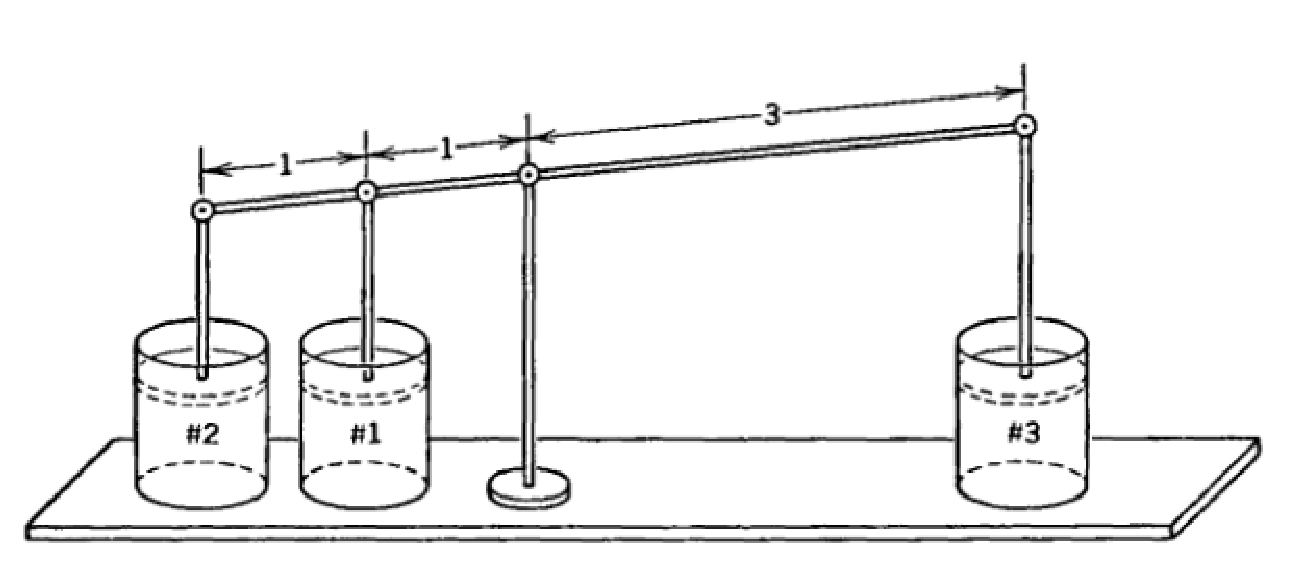
\includegraphics[scale=0.5]{fig2_1.eps} 
	\figcaption{例2.7-1图:三个体积耦合的系统。}
}


{\bf 解}

\ 

{\it 
	封闭性条件要求总能量守恒:
	\[
		\delta U^{(1)} + \delta U^{(2)} + \delta U^{(3)} = 0.
	\]
	活塞之间通过杠杆连接,使得三个圆柱体体积变化的关系为
	\begin{align*}
		\delta V^{(2)} &= 2 \delta V^{(1)} \\
		\delta V^{(3)} &= -3 \delta V^{(1)}
	\end{align*}
	于是熵的极值条件可化为
	\begin{align*}
		\delta S =& \frac{1}{T^{(1)}} \delta U^{(1)} + \frac{1}{T^{(2)}} \delta U^{(2)} + \frac{1}{T^{(3)}} \delta U^{(3)} + \frac{P^{(1)}}{T^{(1)}} \delta V^{(1)} \\
		&+ \frac{P^{(2)}}{T^{(2)}} \delta V^{(2)} + \frac{P^{(3)}}{T^{(3)}} \delta V^{(3)} = 0 \\
		\delta S =& \left( \frac{1}{T^{(1)}} - \frac{1}{T^{(3)}} \right) \delta U^{(1)} + \left( \frac{1}{T^{(2)}} - \frac{1}{T^{(3)}} \right) \delta U^{(2)} \\
		&+ \left( \frac{P^{(1)}}{T^{(1)}} + 2\frac{P^{(2)}}{T^{(2)}} - 3\frac{P^{(3)}}{T^{(3)}} \right) \delta V^{(1)} = 0
	\end{align*}
	$\delta U^{(1)}, \delta U^{(2)}, \delta V^{(1)}$相互独立,可任意取值,因此上式意味着它们的系数均为零。$\delta U^{(1)}$的系数为零可得$T^{(1)} = T^{(3)}$,$\delta U^{(2)}$可得$T^{(2)} = T^{(3)}$,$\delta V^{(1)}$的系数为零结合三个系统温度相等可得
	\[ P^{(1)} + 2P^{(2)} = 3P^{(3)}. \]
	考虑到力学中的杠杆平衡原理,上面的平衡条件在意料之中。若已知状态方程就可将上式化为三个系统体积的等式。
}
\end{example}

\section{存在物质交换时的平衡态}
\label{sec2.8}
化学势的含义要从存在物质流动的情况考虑。设想由不可移动的透热壁分隔的两个简单系统,且第$\alpha$种物质组分\mpar{为避免与子系统编号$\ ^{(1)}, \ ^{(2)}$混淆,本节用希腊字母$\alpha, \beta, \gamma, \dots$标记不同的物质组分,而非采用原书的数字下标。}可以透过壁,其他组分$N_\beta, \dots$不可透过,这个复合系统的平衡态条件是参量$U^{(1)}, U^{(2)}, N_\alpha^{(1)}, N_\alpha^{(2)}$,复合系统熵的微分为
\begin{equation}
	dS = \frac{1}{T^{(1)}} dU^{(1)} - \frac{\mu_\alpha^{(1)}}{T^{(1)}} dN_\alpha^{(1)} + \frac{1}{T^{(2)}} dU^{(2)} - \frac{\mu_\alpha^{(2)}}{T^{(2)}} dN_\alpha^{(2)}
\label{equ2.57}
\end{equation}
封闭性条件为
\begin{align}
	dU^{(2)} &= -dU^{(1)} \label{equ2.58}\\
	dN_\alpha^{(2)} &= - dN_\alpha^{(1)}
\label{equ2.59}
\end{align}
于是
\begin{equation}
	dS = \left( \frac{1}{T^{(1)}} - \frac{1}{T^{(2)}} \right) dU^{(1)} - \left( \frac{\mu_\alpha^{(1)}}{T^{(1)}} - \frac{\mu_\alpha^{(2)}}{T^{(2)}} \right) dN_\alpha^{(1)}.
\label{equ2.60}
\end{equation}
对任意$dU^{(1)}, dN_\alpha^{(1)}$有$dS = 0$,因此平衡条件为
\begin{align}
	\frac{1}{T^{(1)}} = \frac{1}{T^{(2)}} 
\label{equ2.61} \\
	\frac{\mu_\alpha^{(1)}}{T^{(1)}} = \frac{\mu_\alpha^{(2)}}{T^{(2)}}, \quad (\text{因此} \mu_\alpha^{(1)} = \mu_\alpha^{(2)})
\label{equ2.62}
\end{align}
就像温度可以看做热流的“势”,压强为体积变化的“势”那样,化学势可以视为物质流动的“势”。化学势的差值是造成物质流动的“广义力”。

物质流动的方向与化学势的关系可以用\ref{sec2.5}节分析热流的方法导出。设子系统温度相等$T^{(1)} = T^{(2)}$,\eqref{equ2.60}式化为
\begin{equation}
	dS = \frac{\mu_\alpha^{(2)} - \mu_\alpha^{(1)}}{T} dN_\alpha^{(1)}
\label{equ2.63}
\end{equation}
如果$\mu_\alpha^{(1)} > \mu_\alpha^{(2)}$,则由于$dS > 0$, 故而$dN_\alpha^{(1)}< 0$,即物质从高化学势流向低化学势的地方。

之后会看到化学势除了提供物质流动的“广义力”之外,还与物质相变以及化学反应有关,“化学势”的名字正是源自它在理论化学中的重要地位。

化学势的单位是Joule每摩尔(或任意的能量单位每摩尔)。


\section{化学平衡}
\label{sec2.9}
发生化学反应的系统的热力学描述与前面的复合系统相似,它的平衡条件仍然由化学势$\mu$的方程表示——这也是{\it 化学势}名字的来源。

在化学反应过程中,系统物质组分的摩尔数发生变化,有些增加有些减少。摩尔数之间的变化关系由化学反应方程决定,例如
\begin{equation}
	2\ce{H2} + \ce{O2} \leftrightharpoons 2 \ce{H2O}
\label{equ2.64}
\end{equation}
再比如
\begin{equation}
	2\ce{O} \leftrightharpoons \ce{O2}
\label{equ2.65}
\end{equation}
第一个方程里,氢分子、氧分子与水分子变化量之比为$-2 : -1 : +2$. 一般形式是,对于$r$种物质参与的化学反应有:
\begin{equation}
	0 \leftrightharpoons \sum_j \nu_j A_j.
\end{equation}
其中$\nu_j$称为“计量系数 (stoichiometric coefficients)”,例子中氢分子、氧分子与水分子的计量系数分别为$-2, -1, +2$. $A_j$表示化学势,上例中$A_1 = \ce{H2}, A_2 = \ce{O2}, A_3 = \ce{H2O}$. 如果从反方向考虑化学反应(例如水{\it 离解}成氢气氧气),则$\nu_j$反号。$\nu_j$没有绝对的正负性,只有相对的正负才有意义。

系统的基本方程为
\begin{equation}
	S = S(U, V, N_1, N_2, \dots, N_r).
\label{equ2.67}
\end{equation}
假设整个反应体系处于封闭的刚性绝热容器中,系统的总能量$U$,总体积$V$不变。\mpar{这当然不是化学反应最一般的边界条件,一般情况下容器是开放的,可以与外界交换能量,体积也可改变。我们在6.4节讨论这种开放条件下的反应。}

化学反应造成的熵变为
\begin{equation}
	dS = - \sum_{j = 1}^{r} \frac{\mu_j}{T} dN_j.
\label{equ2.68}
\end{equation}
注意,摩尔数的改变与计量系数$\nu_j$成正比,设比例系数为$d\bar{N}$,则
\begin{equation}
	dS = -\frac{d\bar{N}}{T} \sum_{j = 1}^r \mu_j \nu_j
\label{equ2.69}
\end{equation}
因而熵的极值原理表明平衡条件为
\begin{equation}
	\sum_{j = 1}^r \mu_j \nu_j = 0.
\label{equ2.70}
\end{equation}
若系统的状态方程已知,则由平衡条件\eqref{equ2.70}式可以解出平衡状态下各组分的摩尔数。

下面举一个例子。设一个封闭容器内有氢气、氧气与二氧化碳,并进行如下反应:
\begin{equation}
\begin{split}
	\ce{H2} + \frac{1}{2} \ce{O2} &\leftrightharpoons \ce{H2O} \\
	\ce{CO2} + \ce{H2} &\leftrightharpoons \ce{CO} + \ce{H2O} \\
	\ce{CO} + \frac{1}{2} \ce{O2} &\leftrightharpoons \ce{CO2}
\end{split}
\label{equ2.71}
\end{equation}
平衡条件为
\begin{equation}
\begin{split}
	\mu_{\ce{H2}} + \frac{1}{2} \mu_{\ce{O2}} &= \mu_{\ce{H2O}} \\
	\mu_{\ce{CO2}} + \mu_{\ce{H2}} &= \mu_{\ce{CO}} + \mu_{\ce{H2O}} \\
	\mu_{\ce{CO}} + \frac{1}{2} \mu_{\ce{O2}} &= \mu_{\ce{CO2}}
\end{split}
\label{equ2.72}
\end{equation}
上面只有{\it 两个}独立方程(第一个方程是后两个方程的和,第一个化学反应是后两个反应的净结果)。开始反应时氢气、氧气与二氧化碳物质的量之比(可人为控制任意改变)提供另外三个条件。于是有五个未知量(\ce{H2}, \ce{O2}, \ce{H2O}, \ce{CO2}, \ce{CO}的量),五个方程,原则上可以解出。

通常情况在开放容器中的化学反应终态的温度与压强均为定值。因此尽管未知量增加了两个(能量与体积),但$T$与$P$的关系提供了两个新条件,问题同样可以求解。

关于化学反应更详尽的讨论见6.4节。现在只需要记住化学势在物质流动和化学反应中的角色就像温度在热量流动、压强在体积变化中一样。
